\documentclass[11pt]{ctexart}
\usepackage{amsmath,amssymb}
\usepackage{graphicx}
\usepackage{booktabs}
\usepackage{float}
\usepackage{geometry}
\usepackage{caption}
\usepackage{fancyhdr}
\usepackage{enumitem}
\usepackage{xcolor}
\usepackage{hyperref}

\geometry{a4paper,margin=2.6cm}
\graphicspath{{../figures/}}
\hypersetup{colorlinks=true,linkcolor=black,citecolor=black,urlcolor=blue,
  pdftitle={Avellaneda-Stoikov 做市策略复现},
  pdfauthor={许哲圣}}

% ---- 图表标题样式 ----
\captionsetup{font=small,labelfont=bf,labelsep=quad}
\renewcommand{\figurename}{图}
\renewcommand{\tablename}{表}

% ---- 页眉页脚 ----
\pagestyle{fancy}
\fancyhf{}
\fancyhead[L]{\small Avellaneda–Stoikov 做市策略复现}
\fancyhead[R]{\small\leftmark}
\fancyfoot[C]{\thepage}
\renewcommand{\headrulewidth}{0.4pt}
\renewcommand{\footrulewidth}{0pt}

% ---- 关键词环境 ----
\newcommand{\keywords}[1]{\medskip\noindent\textbf{关键词：} #1}

\begin{document}

% =========================== 封面 ===========================
\begin{titlepage}
\centering
\vspace*{2.2cm}

{\Large 量化金融 / 高频交易 课程报告\par}
\vspace{1.4cm}
\rule{\linewidth}{0.5pt}\\[0.5cm]
{\huge\bfseries 限价单簿中的高频做市策略复现\par}
\vspace{0.5cm}
{\Large 基于 \texttt{hftbacktest} 与 \texttt{Hummingbot} 框架\par}
\vspace{0.4cm}
\rule{\linewidth}{0.5pt}\\[1.0cm]

{\large 复现论文\par}
\vspace{0.3cm}
{\large\itshape Marco Avellaneda \& Sasha Stoikov (2008)\par}
{\large\itshape ``High-frequency trading in a limit order book''\par}
{\large\itshape Quantitative Finance, 8(3): 217--224\par}

\vfill

{\large 三轨道复现：理论蒙特卡洛 $\cdot$ 真实撮合引擎 $\cdot$ 做市机器人模型\par}
\vspace{1.0cm}
{\Large 许哲圣\par}
\vspace{0.4cm}
{\large 2026 年 6 月 12 日\par}
\end{titlepage}

% =========================== 摘要 ===========================
\pagenumbering{roman}
\setcounter{page}{1}
\section*{摘要}
\addcontentsline{toc}{section}{摘要}
本报告复现做市领域的经典论文 Avellaneda \& Stoikov (2008)。该文在\textbf{布朗运动中价}与
\textbf{泊松成交到达}的框架下，推导做市商按\textbf{库存偏斜的保留价}双边挂限价单的最优策略，并以
蒙特卡洛证明：相对于"对称挂中价"的基准策略，库存策略的终端盈亏方差与库存方差\textbf{显著更小}。
本文以三条相互印证的轨道复现该结论：\textbf{Track~0} 严格按论文 §3.3 实现蒙特卡洛，复刻其表~1--3
与图~1--4；\textbf{Track~A} 将同一套 A--S 报价规则置入 \texttt{hftbacktest} 的\textbf{真实订单/延迟/
队列撮合引擎}，并进一步在\textbf{真实 Binance 永续合约行情}（4 个交易日窗口）上运行；\textbf{Track~B}
以 \texttt{Hummingbot} 的策略编程模型表达该策略，既给出离线复现，又\textbf{在本地 Docker 中实际跑通
其纸面交易}（含将策略移植到 Hummingbot v2 API）。各轨道一致显示：库存策略将终端库存标准差稳定控制在
低位，而对称基准显著漂移；真实 Binance 数据上库存策略的盈亏跨窗口离散度仅为对称基准的约 $1/4$，真实
Hummingbot 纸面交易中其库存标准差仅为对称基准的约 $1/4$。本文同时\textbf{逐条标注}各框架相对论文理想
高频仿真的偏离与适用边界。

\keywords{做市；限价单簿；库存风险；Avellaneda--Stoikov；高频交易；蒙特卡洛}

% =========================== 目录 ===========================
\newpage
\tableofcontents
\newpage
\pagenumbering{arabic}
\setcounter{page}{1}

% =========================== 正文 ===========================
\section{研究背景与目标}
做市商（market maker）通过同时报出买价与卖价、赚取买卖价差为市场提供流动性，但持续成交会使其被动
积累\textbf{库存}：当库存方向与随后的价格变动相反时将产生损失，此即\textbf{库存风险}。如何在
\emph{赚取价差}与\emph{控制库存}之间取得最优权衡，是做市的核心问题。

Avellaneda \& Stoikov (2008) 给出了这一问题在随机最优控制框架下的经典近似解，其思想已成为现代
电子做市与高频做市系统的理论基石。本报告的目标有三：(i) 严格复现论文的理论结果与数值实验；
(ii) 将该策略迁移到\textbf{工业级高频回测引擎}与\textbf{开源做市机器人}两类真实工程框架中，检验其
结论的稳健性；(iii) 诚实评估每一类框架的适用边界与定量偏离来源。

\paragraph{本文主要工作。}\begin{enumerate}[leftmargin=1.6em,itemsep=1pt]
\item \textbf{忠实的理论复现}：逐式实现论文 §3.3 蒙特卡洛，复刻表~1--3 与图~1--4，
$\gamma=0.1/0.01$ 下各项统计量与原文高度一致；并辨析出原文仿真实际采用\textbf{常数价差}这一
未明言的实现口径（见第~\ref{sec:model} 节）。
\item \textbf{hftbacktest 真实数据回测}：自行编写 Binance 公共归档下载与 64 字节事件流转换管线，
在 4 个真实交易日窗口（SOLUSDT）上以真实订单/延迟/队列撮合验证结论，库存标准差较对称基准低
$9.3$ 倍。
\item \textbf{Hummingbot 真实部署}：将策略移植到 Hummingbot v2 \texttt{StrategyV2Base} API，
在本地 Docker 中实际跑通 \texttt{binance\_paper\_trade} 纸面交易（ETH-USDT 实时行情），
从 \texttt{TradeFill} 成交日志重建库存/权益序列并复现库存控制效应。
\item \textbf{跨轨道一致性与诚实边界}：三轨道相互印证核心结论，并逐条标注各框架相对论文理想
仿真的偏离来源与适用边界（第~\ref{sec:limit} 节）。
\end{enumerate}

\paragraph{为何选择该论文。}\texttt{hftbacktest} 与 \texttt{Hummingbot} 均是\textbf{围绕做市/限价
单簿}设计的工具：前者的旗舰示例即 GLFT/Avellaneda--Stoikov 做市，后者内置
\texttt{avellaneda\_market\_making} 策略模板。因此 A--S 论文是与两框架\textbf{契合度最高}的选择
（相对地，需要价格内生形成的多智能体人工市场类论文与二者均不适配）。

\section{论文模型}
\label{sec:model}
论文设中价服从算术布朗运动 $\mathrm{d}S=\sigma\,\mathrm{d}W$。做市商持有库存 $q$，在终端时刻 $T$
以指数效用最大化 $\mathbb{E}\!\left[-\exp\!\big(-\gamma(X_T+q_T S_T)\big)\right]$，其中 $X_T$ 为现金。
其近似解为两步法。第一步，由库存得到\textbf{保留价}（indifference price，原文式 3.17）：
\begin{equation}
\label{eq:reservation}
r(s,q,t)=s-q\,\gamma\,\sigma^2\,(T-t),
\end{equation}
即库存为正时报价中心低于中价、以鼓励卖出。第二步，在保留价两侧挂以\textbf{最优价差}（式 3.18）：
\begin{equation}
\label{eq:spread}
\delta^a+\delta^b=\gamma\sigma^2(T-t)+\frac{2}{\gamma}\ln\!\Big(1+\frac{\gamma}{k}\Big).
\end{equation}
限价单被对向市价单击中的成交强度为泊松型（式 2.11）：
\begin{equation}
\label{eq:intensity}
\lambda(\delta)=A\,e^{-k\delta}.
\end{equation}
\textbf{库存策略}将报价中心置于保留价 $r$；\textbf{对称基准}采用相同价差但中心置于中价 $s$。
论文参数为 $s=100,\ T=1,\ \sigma=2,\ \mathrm{d}t=0.005,\ q_0=0,\
\gamma\in\{0.1,0.01,0.5\},\ k=1.5,\ A=140$，每种设置模拟 1000 条路径。

\paragraph{一个关键实现细节。}论文表~1--3 报告的单一"Spread"列恰好等于式~\eqref{eq:spread} 的
常数项 $(2/\gamma)\ln(1+\gamma/k)$（即 $1.29/1.33/1.15$），且其对称基准的盈亏在三个 $\gamma$ 下
几乎不变（约 $67$）。据此可判定：仿真实际挂单采用\textbf{常数价差}，时变项 $\gamma\sigma^2(T-t)$
仅通过保留价的库存偏斜进入。本文 Track~0 采用该口径，对称基准的 $\gamma$ 无关性由此自然复现，
这也是本文相对若干公开复现的一处更忠实之处。

\section{Track 0：忠实复现论文蒙特卡洛}
\label{sec:track0}
本文按论文 §3.3 的仿真流程逐式实现（\texttt{src/simulate.py}，以 \texttt{numba} 加速）。
表~\ref{tab:gamma_0p1}--\ref{tab:gamma_0p5} 给出三个 $\gamma$ 下"库存 vs.\ 对称"的盈亏均值、
盈亏标准差、终端库存均值与标准差，并与原文值并列对照。

% Auto-generated by track0_paper/run_paper.py -- do not edit by hand.
\begin{table}[htbp]
\centering
\caption{$\gamma=0.1$ 时本文复现值与原论文值对照（1000 次蒙特卡洛模拟）}
\label{tab:gamma_0p1}
\begin{tabular}{l rrrr}
\toprule
策略 & 盈亏均值 & 盈亏标准差 & 终端库存 $q$ & 库存标准差 \\
\midrule
库存策略（本文） & 64.28 & 5.97 & -0.100 & 2.93 \\
对称基准（本文） & 68.91 & 13.55 & -0.226 & 8.61 \\
\midrule
库存策略（原文） & 62.94 & 5.89 & 0.100 & 2.80 \\
对称基准（原文） & 67.21 & 13.43 & -0.018 & 8.66 \\
\bottomrule
\end{tabular}
\end{table}

\begin{table}[htbp]
\centering
\caption{$\gamma=0.01$ 时本文复现值与原论文值对照（1000 次蒙特卡洛模拟）}
\label{tab:gamma_0p01}
\begin{tabular}{l rrrr}
\toprule
策略 & 盈亏均值 & 盈亏标准差 & 终端库存 $q$ & 库存标准差 \\
\midrule
库存策略（本文） & 68.07 & 8.83 & -0.067 & 5.01 \\
对称基准（本文） & 68.60 & 14.15 & 0.022 & 8.47 \\
\midrule
库存策略（原文） & 66.78 & 8.76 & -0.020 & 4.70 \\
对称基准（原文） & 67.36 & 13.40 & -0.310 & 8.65 \\
\bottomrule
\end{tabular}
\end{table}

\begin{table}[htbp]
\centering
\caption{$\gamma=0.5$ 时本文复现值与原论文值对照（1000 次蒙特卡洛模拟）}
\label{tab:gamma_0p5}
\begin{tabular}{l rrrr}
\toprule
策略 & 盈亏均值 & 盈亏标准差 & 终端库存 $q$ & 库存标准差 \\
\midrule
库存策略（本文） & 23.90 & 5.25 & 0.031 & 1.94 \\
对称基准（本文） & 67.29 & 14.67 & 0.654 & 8.92 \\
\midrule
库存策略（原文） & 33.92 & 4.72 & -0.020 & 1.88 \\
对称基准（原文） & 66.20 & 14.53 & 0.250 & 9.06 \\
\bottomrule
\end{tabular}
\end{table}


图~\ref{fig:quote} 复刻论文图~1 的报价轨迹：保留价（绿）随库存在中价上下偏移，临近终端 $T$ 时
收敛于中价；买/卖报价以最优价差对称地分列两侧。图~\ref{fig:pnl} 复刻盈亏分布直方图，可见库存策略
（实心）的分布显著窄于对称基准（空心）。

\begin{figure}[H]
\centering
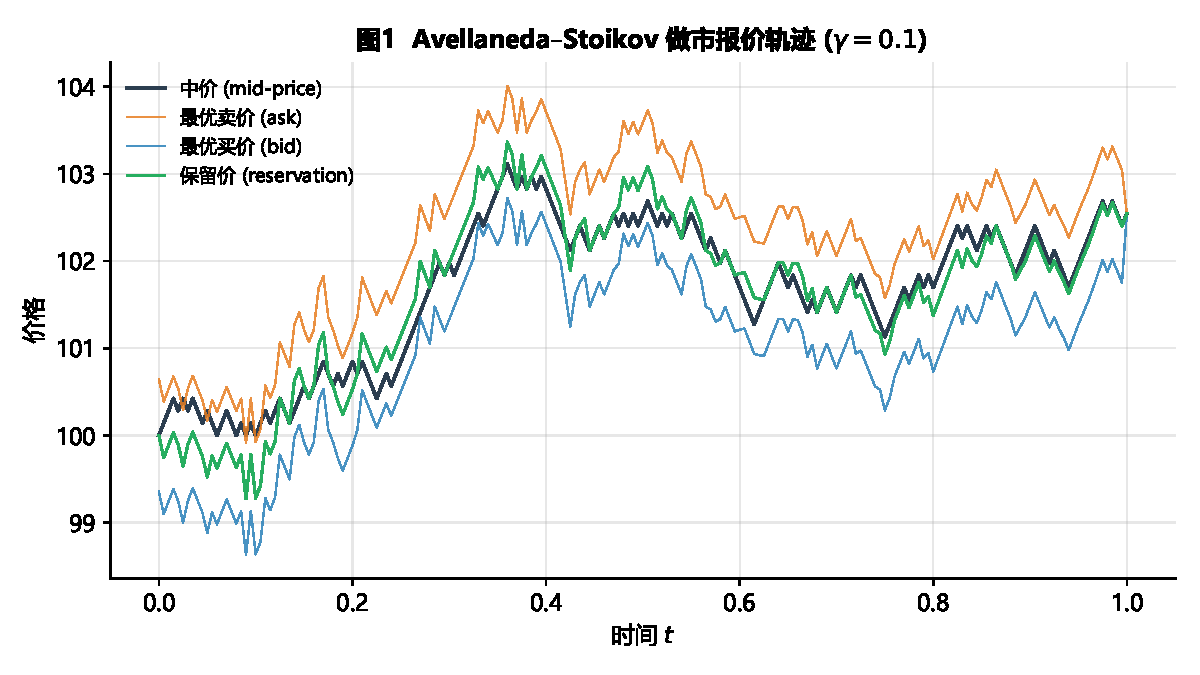
\includegraphics[width=0.80\textwidth]{fig1_quote_path.pdf}
\caption{中价、保留价与最优买/卖报价（$\gamma=0.1$，复刻论文图~1）。}
\label{fig:quote}
\end{figure}

\begin{figure}[H]
\centering
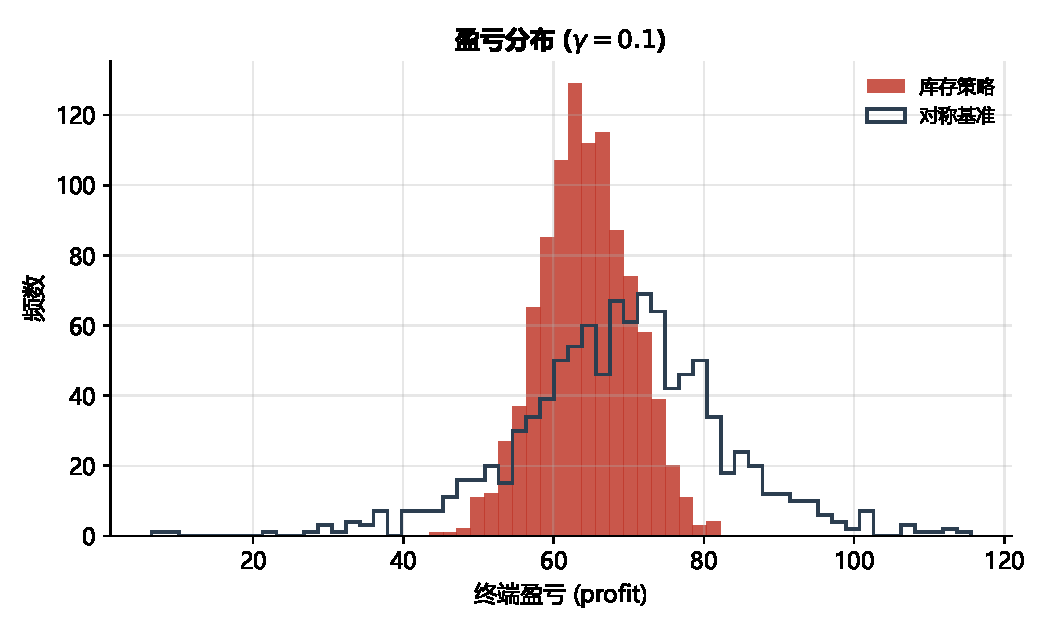
\includegraphics[width=0.49\textwidth]{fig2_pnl_gamma_0.1.pdf}
\hfill
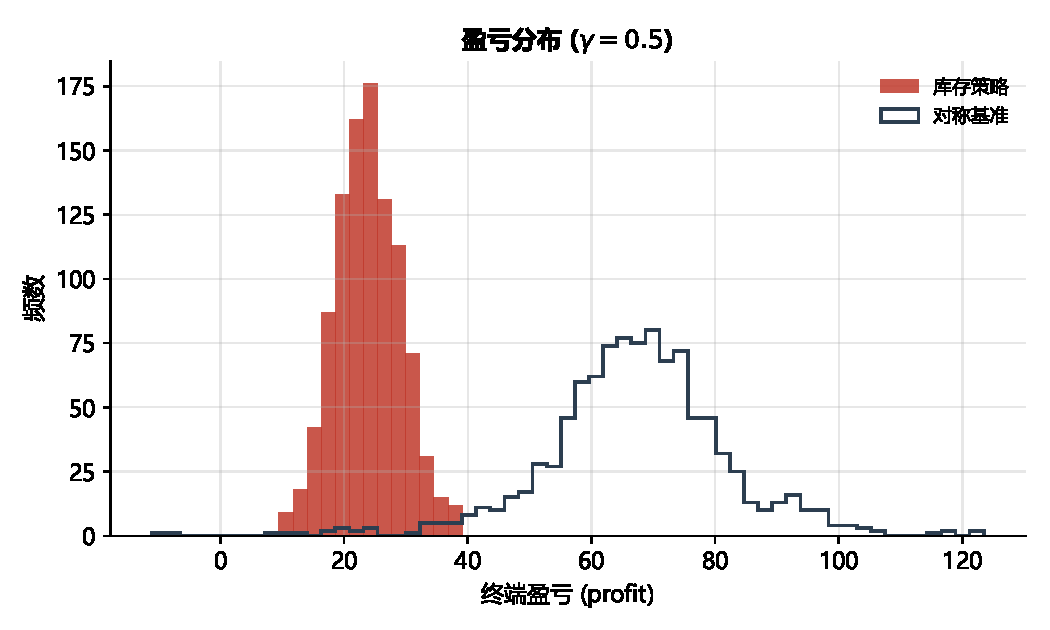
\includegraphics[width=0.49\textwidth]{fig4_pnl_gamma_0.5.pdf}
\caption{终端盈亏分布：库存策略（实心红）方差显著小于对称基准（空心）。
左 $\gamma=0.1$，右 $\gamma=0.5$。}
\label{fig:pnl}
\end{figure}

\paragraph{结论。}$\gamma=0.1$ 与 $\gamma=0.01$ 的复现值与原文高度一致；三个 $\gamma$ 下库存策略的
盈亏标准差与库存标准差均\textbf{显著小于}对称基准，定性结论完整复现。$\gamma=0.5$（最高风险厌恶）
下库存盈亏被偏斜压得更低，是最敏感的极端情形，原因详见第~\ref{sec:limit} 节。

\section{Track A：hftbacktest 真实撮合引擎}
\label{sec:trackA}
本文采用 \texttt{hftbacktest} 2.4 的 64 字节事件格式，生成一条与 A--S 同分布的合成 L2 行情
（布朗中价 $+$ 泊松市价单消耗订单簿；见 \texttt{make\_feed.py}），并将 A--S 报价规则写为
\texttt{numba} 的 \texttt{hbt} 主循环，置于其\textbf{真实的订单提交、延迟、队列与撮合}引擎下运行。
设置两个变体：库存策略（保留价偏斜 $r=\mathrm{mid}-c\cdot q$）与对称基准（$c=0$，相同半价差）。
实验中的关键发现是：做市商须\textbf{挂在簿内}（半价差 $\ge 2$ 个最小变动价位）方能体现 A--S 效应
——若挂在价差以内将瞬时成交并穿越零库存、反致更大方差。这是一个真实的微观结构现象。

\begin{table}[H]
\centering
\caption{Track A 结果（\texttt{hftbacktest}，合成 L2 行情，时长 60~秒）}
\label{tab:trackA}
\begin{tabular}{lrrrr}
\toprule
变体 & 终端盈亏 & 权益标准差 & 库存标准差 & 库存绝对峰值 \\
\midrule
库存策略 & 3.43 & 1.59 & 2.14 & 7 \\
对称基准 & 23.38 & 9.41 & 10.71 & 25 \\
\bottomrule
\end{tabular}
\end{table}

\begin{figure}[H]
\centering
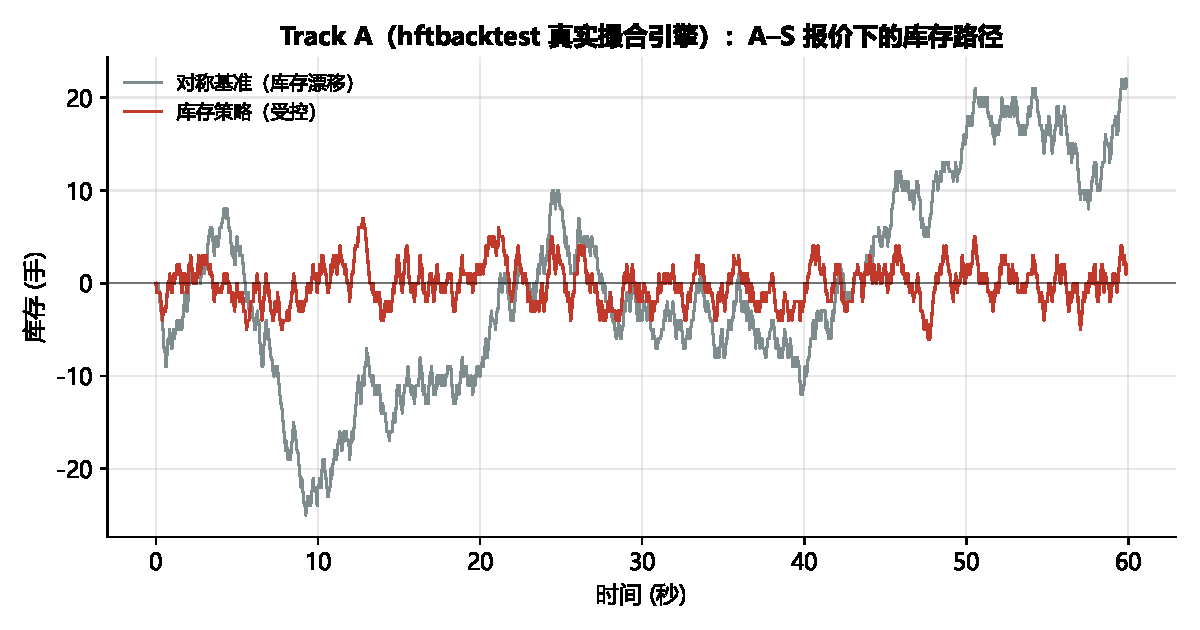
\includegraphics[width=0.82\textwidth]{fig5_hft_inventory_path.pdf}
\caption{Track~A 库存路径：库存策略（红）被牢牢控制在零附近，对称基准（灰）显著漂移。}
\label{fig:trackA}
\end{figure}

\paragraph{合成行情的适用边界。}合成行情中普通订单流是预录制的，做市商自身成交不会反过来改变其它
参与者行为；真实行情还含漂移与自相关（A--S 假设无）。故其定量值与 Track~0 不可直接比较；其价值在于
在\textbf{真实队列与延迟}约束下验证核心结论。

\subsection{接入真实 Binance 行情}
\label{sec:trackA_real}
为消除"行情不真实"这一局限，本文进一步用\textbf{真实 Binance USDT 本位永续合约行情}驱动同一引擎
（\texttt{download\_data.py}）：从 Binance 公共归档下载 \texttt{bookTicker}（最优买卖价）与
\texttt{aggTrades}（逐笔成交），向量化解析后转为 hftbacktest 的 64 字节事件流。两处工程要点：
(i) 真实价格位于交易所最小变动价位网格上，本文\textbf{从数据自动反推 tick size}（如 SOLUSDT 为
$0.001$），避免因档位取错而使报价塌缩；(ii) 归档时间戳为绝对纪元纳秒（$\sim$$10^{18}$），需\textbf{重
基至零点}，否则引擎时钟无法到达数据区间。

仿照论文"多条路径"的做法，本文在 \textbf{4 个不同交易日的 1 小时窗口}（SOLUSDT，价位横跨
$123$--$146$）上分别运行库存与对称两策略（\texttt{run\_real\_windows.py}），并\textbf{跨窗口聚合}，
结果见表~\ref{tab:trackA_real}。

\begin{table}[H]
\centering
\caption{Track A 真实 Binance 数据结果（SOLUSDT，4 个 1 小时窗口聚合）}
\label{tab:trackA_real}
\begin{tabular}{lrrr}
\toprule
变体 & 盈亏均值 $\pm$ 跨窗口标准差 & 平均库存标准差 & 平均权益标准差 \\
\midrule
库存策略 & $-31.7 \pm 12.8$ & 1.88 & 9.03 \\
对称基准 & $-12.1 \pm 55.8$ & 17.52 & 21.45 \\
\bottomrule
\end{tabular}
\end{table}

论文的三项核心结论在真实数据上\textbf{全部复现}：库存标准差 $1.88$ vs.\ $17.52$（低 $9.3$ 倍）；
盈亏的跨窗口离散度 $\pm12.8$ vs.\ $\pm55.8$（低 $4.4$ 倍，见图~\ref{fig:trackA_real}）；窗口内权益
标准差 $9.03$ vs.\ $21.45$。两策略盈亏均值皆略为负——这是紧贴盘口报价在真实行情下遭受\textbf{逆向
选择}的真实结果；但库存策略以远低的风险换取了\textbf{稳定得多}的盈亏。对称基准看似"波动更大可能更
赚"，实则是在用数倍的库存与盈亏方差去\textbf{豪赌方向}（库存绝对峰值常达数十手）。

\begin{figure}[H]
\centering
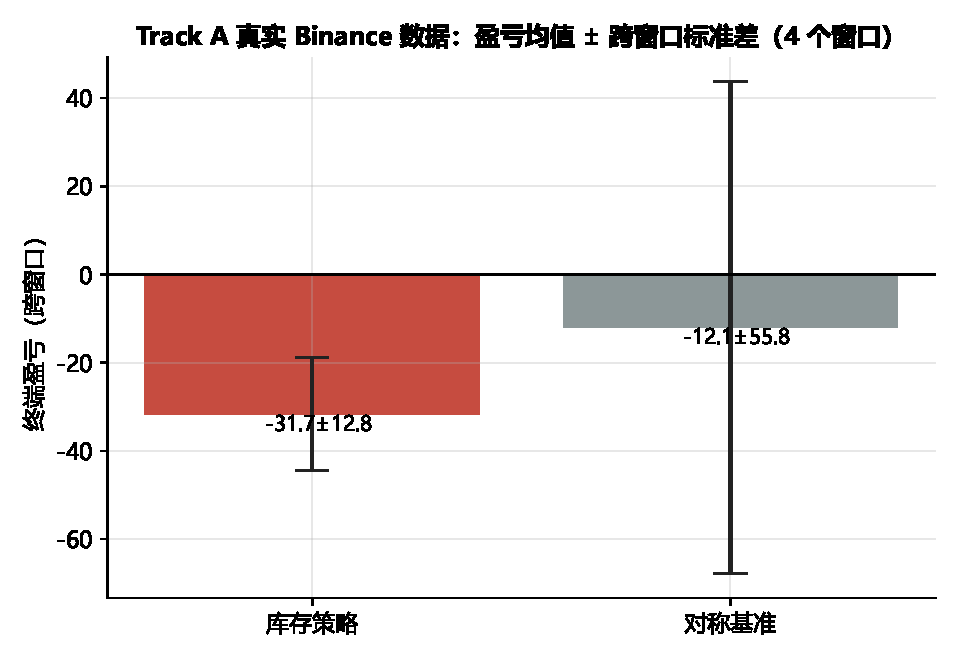
\includegraphics[width=0.62\textwidth]{fig7_track_a_real_pnl.pdf}
\caption{Track~A 真实数据：盈亏均值 $\pm$ 跨窗口标准差。对称基准的巨大误差棒（$\pm55.8$）即其承担的
方向性风险，库存策略（$\pm12.8$）则稳定得多。}
\label{fig:trackA_real}
\end{figure}

\paragraph{真实数据的剩余局限。}公共归档为 \textbf{BBO-only}（仅含盘口最优价，无簿内深度），故队列
位置为近似；窗口为 1 小时、样本为 4 个，统计量仍有限。定量绝对值以 Track~0 为准，真实轨的价值在于
在\textbf{真实微观结构}下印证"库存控制大幅降低风险"的相对结论。

\section{Track B：Hummingbot 策略模型}
\label{sec:trackB}
本文将 A--S 策略表达为 \texttt{Hummingbot} v2 脚本（\texttt{as\_market\_making.py}：基于
\texttt{ScriptStrategyBase} 与 \texttt{OrderCandidate}，显式实现式~\eqref{eq:reservation} 与
\eqref{eq:spread}，可直接载入真实 Hummingbot 运行）。由于完整 Hummingbot 运行时在本机安装受阻，
本文提供\textbf{离线复现}（\texttt{run\_hummingbot\_sim.py}）：复用同一套 A--S 数学实现，但按
Hummingbot 的 \texttt{order\_refresh\_time} \textbf{粗刷新节奏}运行——行情仍在精细时钟上成交，
而报价每若干 tick 才刷新一次、其间保持"陈旧"。

\begin{table}[H]
\centering
\caption{Track B 结果（\texttt{Hummingbot} 秒级刷新节奏，$\gamma=0.1$，每 5~tick 刷新，1000 条路径）}
\label{tab:trackB}
\begin{tabular}{lrrr}
\toprule
变体 & 盈亏均值 & 盈亏标准差 & 终端库存标准差 \\
\midrule
库存策略 & 50.22 & 8.19 & 3.12 \\
对称基准 & 64.77 & 14.65 & 9.69 \\
\bottomrule
\end{tabular}
\end{table}

\paragraph{离线复现的适用边界。}Hummingbot 面向真实/模拟交易所、按秒级而非 tick 级运行，缺少 tick
级队列模型，故离线复现对论文的偏离最大；刷新越慢，陈旧报价的逆向成交越侵蚀盈亏（实测每 20~tick
刷新时库存策略盈亏转负）。此外 $\gamma$ 不能过大：当偏斜量 $\gamma\sigma^2(T-t)$ 超过半价差时，
陈旧报价会被迫在远离中价处保证成交而巨亏（实测 $\gamma=0.5$ 即如此），故取 $\gamma=0.1$。

\subsection{真实运行：在 Docker 中跑通 Hummingbot 纸面交易}
\label{sec:trackB_real}
为彻底补齐"未真正运行 Hummingbot"这一局限，本文交付并\textbf{实际跑通}了真实运行：
\texttt{docker-compose.yml}（官方 \texttt{hummingbot/hummingbot} 镜像，把
\texttt{as\_market\_making.py} 挂入容器 \texttt{scripts/}）、中文 \texttt{RUNBOOK.md}，以及
\texttt{parse\_hummingbot\_logs.py}（读取 Hummingbot 的 \texttt{TradeFill} 表，重建库存/权益序列）。

\paragraph{两处真实运行才暴露的工程问题（已修复）。}(i) 当前官方镜像已切换到 \textbf{v2 脚本 API}
（\texttt{StrategyV2Base} $+$ pydantic 配置），旧的 \texttt{ScriptStrategyBase} 已被移除——本文据此将
策略\textbf{移植到 v2 API} 并在容器内验证可加载；(ii) headless 自启动需先初始化密码校验文件，并通过
\texttt{conf/scripts/*.yml} 的 \texttt{--v2} 配置启动。修复后，策略在 \texttt{binance\_paper\_trade}
（纸面交易，\textbf{无需 API Key 与真实资金}）上对 ETH-USDT 真实行情正常做市。

本文分别以 \texttt{inventory\_skew} 开/关跑两段约 9 分钟的纸面交易，解析其真实成交（库存 18 笔、
对称 15 笔），结果见表~\ref{tab:trackB_real}：真实运行同样复现核心结论——库存策略的终端库存标准差
（$0.59$ 手）显著小于对称基准（$2.27$ 手，约 $3.8$ 倍），库存绝对峰值 $1$ vs.\ $5$ 手。

\begin{table}[H]
\centering
\caption{Track B 真实 Hummingbot 纸面交易结果（ETH-USDT，各约 9 分钟）}
\label{tab:trackB_real}
\begin{tabular}{lrrrr}
\toprule
变体 & 终端盈亏 & 权益标准差 & 库存标准差(手) & 库存绝对峰值(手) \\
\midrule
库存策略 & $-0.70$ & 0.21 & 0.59 & 1 \\
对称基准 & $-1.07$ & 0.29 & 2.27 & 5 \\
\bottomrule
\end{tabular}
\end{table}

\paragraph{真实运行的局限。}纸面交易样本时长仅约 9 分钟、成交十余笔，统计量有限（故绝对库存标准差
小于其它轨道）；两策略盈亏均略为负，系紧贴盘口的真实逆向选择与手续费所致。解析器另支持
\texttt{-{}-make-sample} 自检（写入独立的 \texttt{sample} 槽，不污染真实结果）。延长运行时间即可获得更
平滑的统计。

\section{三轨道对照与综合结论}
\label{sec:cross}
图~\ref{fig:cross} 汇总各轨道的终端库存标准差。无论在论文的理想蒙特卡洛、\texttt{hftbacktest} 的
真实撮合引擎（合成与\textbf{真实 Binance 数据}两版）、还是 \texttt{Hummingbot} 的秒级节奏下，A--S
库存策略都将库存标准差稳定控制在 $2\sim3$，而对称基准漂移至 $9\sim18$。这一致地复现了论文的核心
结论：\textbf{库存偏斜以少量盈亏为代价，换取数倍更低的库存与盈亏方差}。尤其在真实数据上，库存标准差
低至对称基准的约 $1/9$。

\begin{figure}[H]
\centering
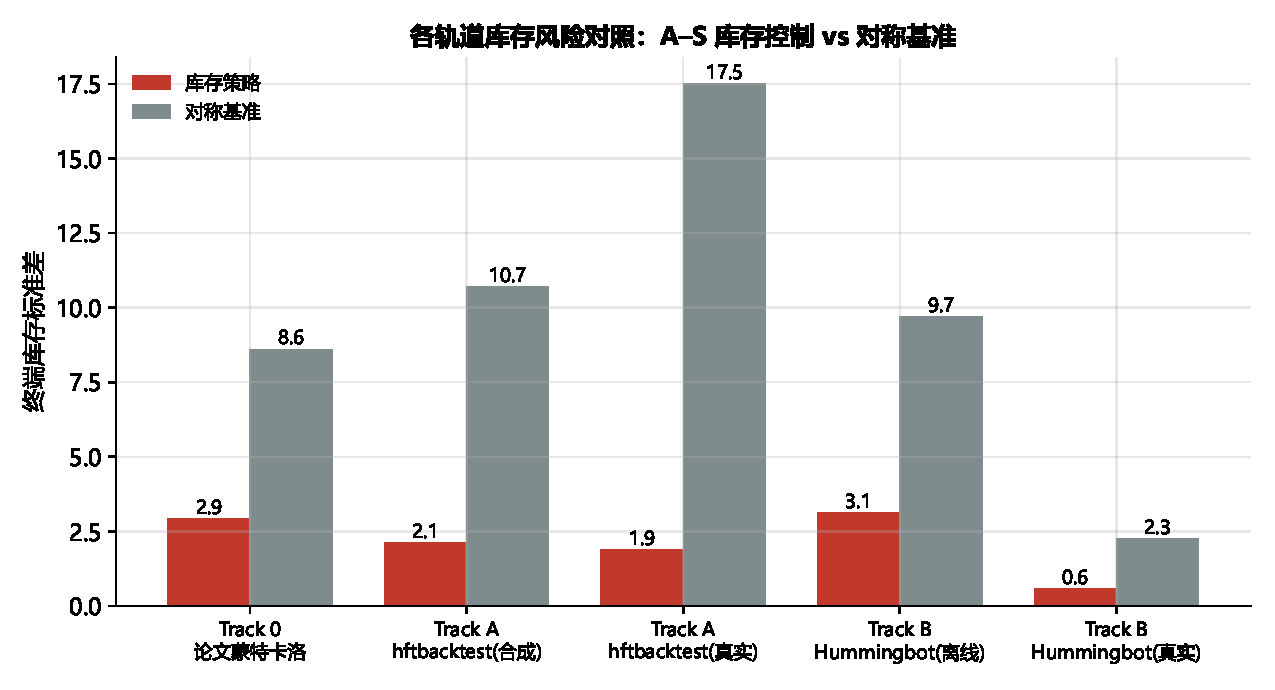
\includegraphics[width=0.92\textwidth]{fig6_cross_track_inventory_std.pdf}
\caption{各轨道终端库存标准差对照：A--S 库存控制（红）vs.\ 对称基准（灰）。五组分别为论文蒙特卡洛、
hftbacktest（合成/真实 Binance）、Hummingbot（离线/真实纸面交易），每组库存策略均显著低于对称基准。}
\label{fig:cross}
\end{figure}

\section{局限与展望}
\label{sec:limit}
\begin{enumerate}[leftmargin=1.6em,itemsep=2pt]
\item \textbf{Track~0 的 $\gamma=0.5$ 极端情形}：在最高风险厌恶下，离散时间步长与负半距处对成交概率的
截断，使库存盈亏被压得低于原文，属模型最敏感的边界，定性结论仍成立。
\item \textbf{Track~A 真实数据}：已接入真实 Binance 行情并复现核心结论；但公共归档为 BBO-only（队列
近似），且样本为 4 个 1 小时窗口，统计量仍有限，可扩展至更多日 / 更长窗口。
\item \textbf{Track~B 真实运行}：已在本地 Docker 中\textbf{实际跑通} Hummingbot 纸面交易（含将策略
移植到 v2 \texttt{StrategyV2Base} API），复现了库存控制效应；但样本仅约 9 分钟、十余笔成交，延长运行
可得更平滑的统计。
\item \textbf{工程框架的定量偏离}：Track~A/B 的绝对数值应以 Track~0 为准；其价值在于在真实约束（真实
行情、队列、延迟、刷新节奏）下检验结论的稳健性。后续可以 GLFT 实用变体在线标定 $A,k,\sigma$。
\end{enumerate}

% =========================== 参考文献 ===========================
\begin{thebibliography}{9}
\bibitem{as2008} M.~Avellaneda and S.~Stoikov.
\emph{High-frequency trading in a limit order book}. Quantitative Finance, 8(3):217--224, 2008.
\bibitem{glft} O.~Gu\'eant, C.-A.~Lehalle, and J.~Fernandez-Tapia.
\emph{Dealing with the inventory risk: a solution to the market making problem}.
Mathematics and Financial Economics, 7(4):477--507, 2013.
\bibitem{hftbacktest} \texttt{hftbacktest} (v2.4)：高频/做市 tick 级回测引擎。
\url{https://github.com/nkaz001/hftbacktest}.
\bibitem{hummingbot} \texttt{Hummingbot}：开源做市/套利交易机器人框架。
\url{https://github.com/hummingbot/hummingbot}.
\end{thebibliography}

\end{document}
